In the experiments using HEPMiner, AFGMiner-locreg was always faster than AFGMiner-iso. As an example, when running with MMH and MinSup of 0.001, AFGMiner-iso took approximately 11 hours to complete the mining process, while AFGMiner-locreg took 40 minutes and p-AFGMiner with 8 threads took 15 minutes. The dramatic decrease in run-time when comparing AFGMiner-locreg to AFGMiner-iso is expected because location registration decreases the number of dataset sub-graphs that must be tested for isomorphism with candidate patterns. 

We also compared patterns found by AFGMiner and FlowGSP. Figure~\ref{fig:NumPatterns} shows the number of output patterns for different MinSup values. As expected, AFGMiner found all patterns found by FlowGSP, but also found additional patterns composed of multiple sub-paths. For flat profiles, the trend is for AFGMiner to find many more patterns than FlowGSP as the MinSup is decreased, with the sequential patterns found by both being the parent patterns of the sub-graph patterns found exclusively by AFGMiner. 

\begin{figure}[h!]
\centering
    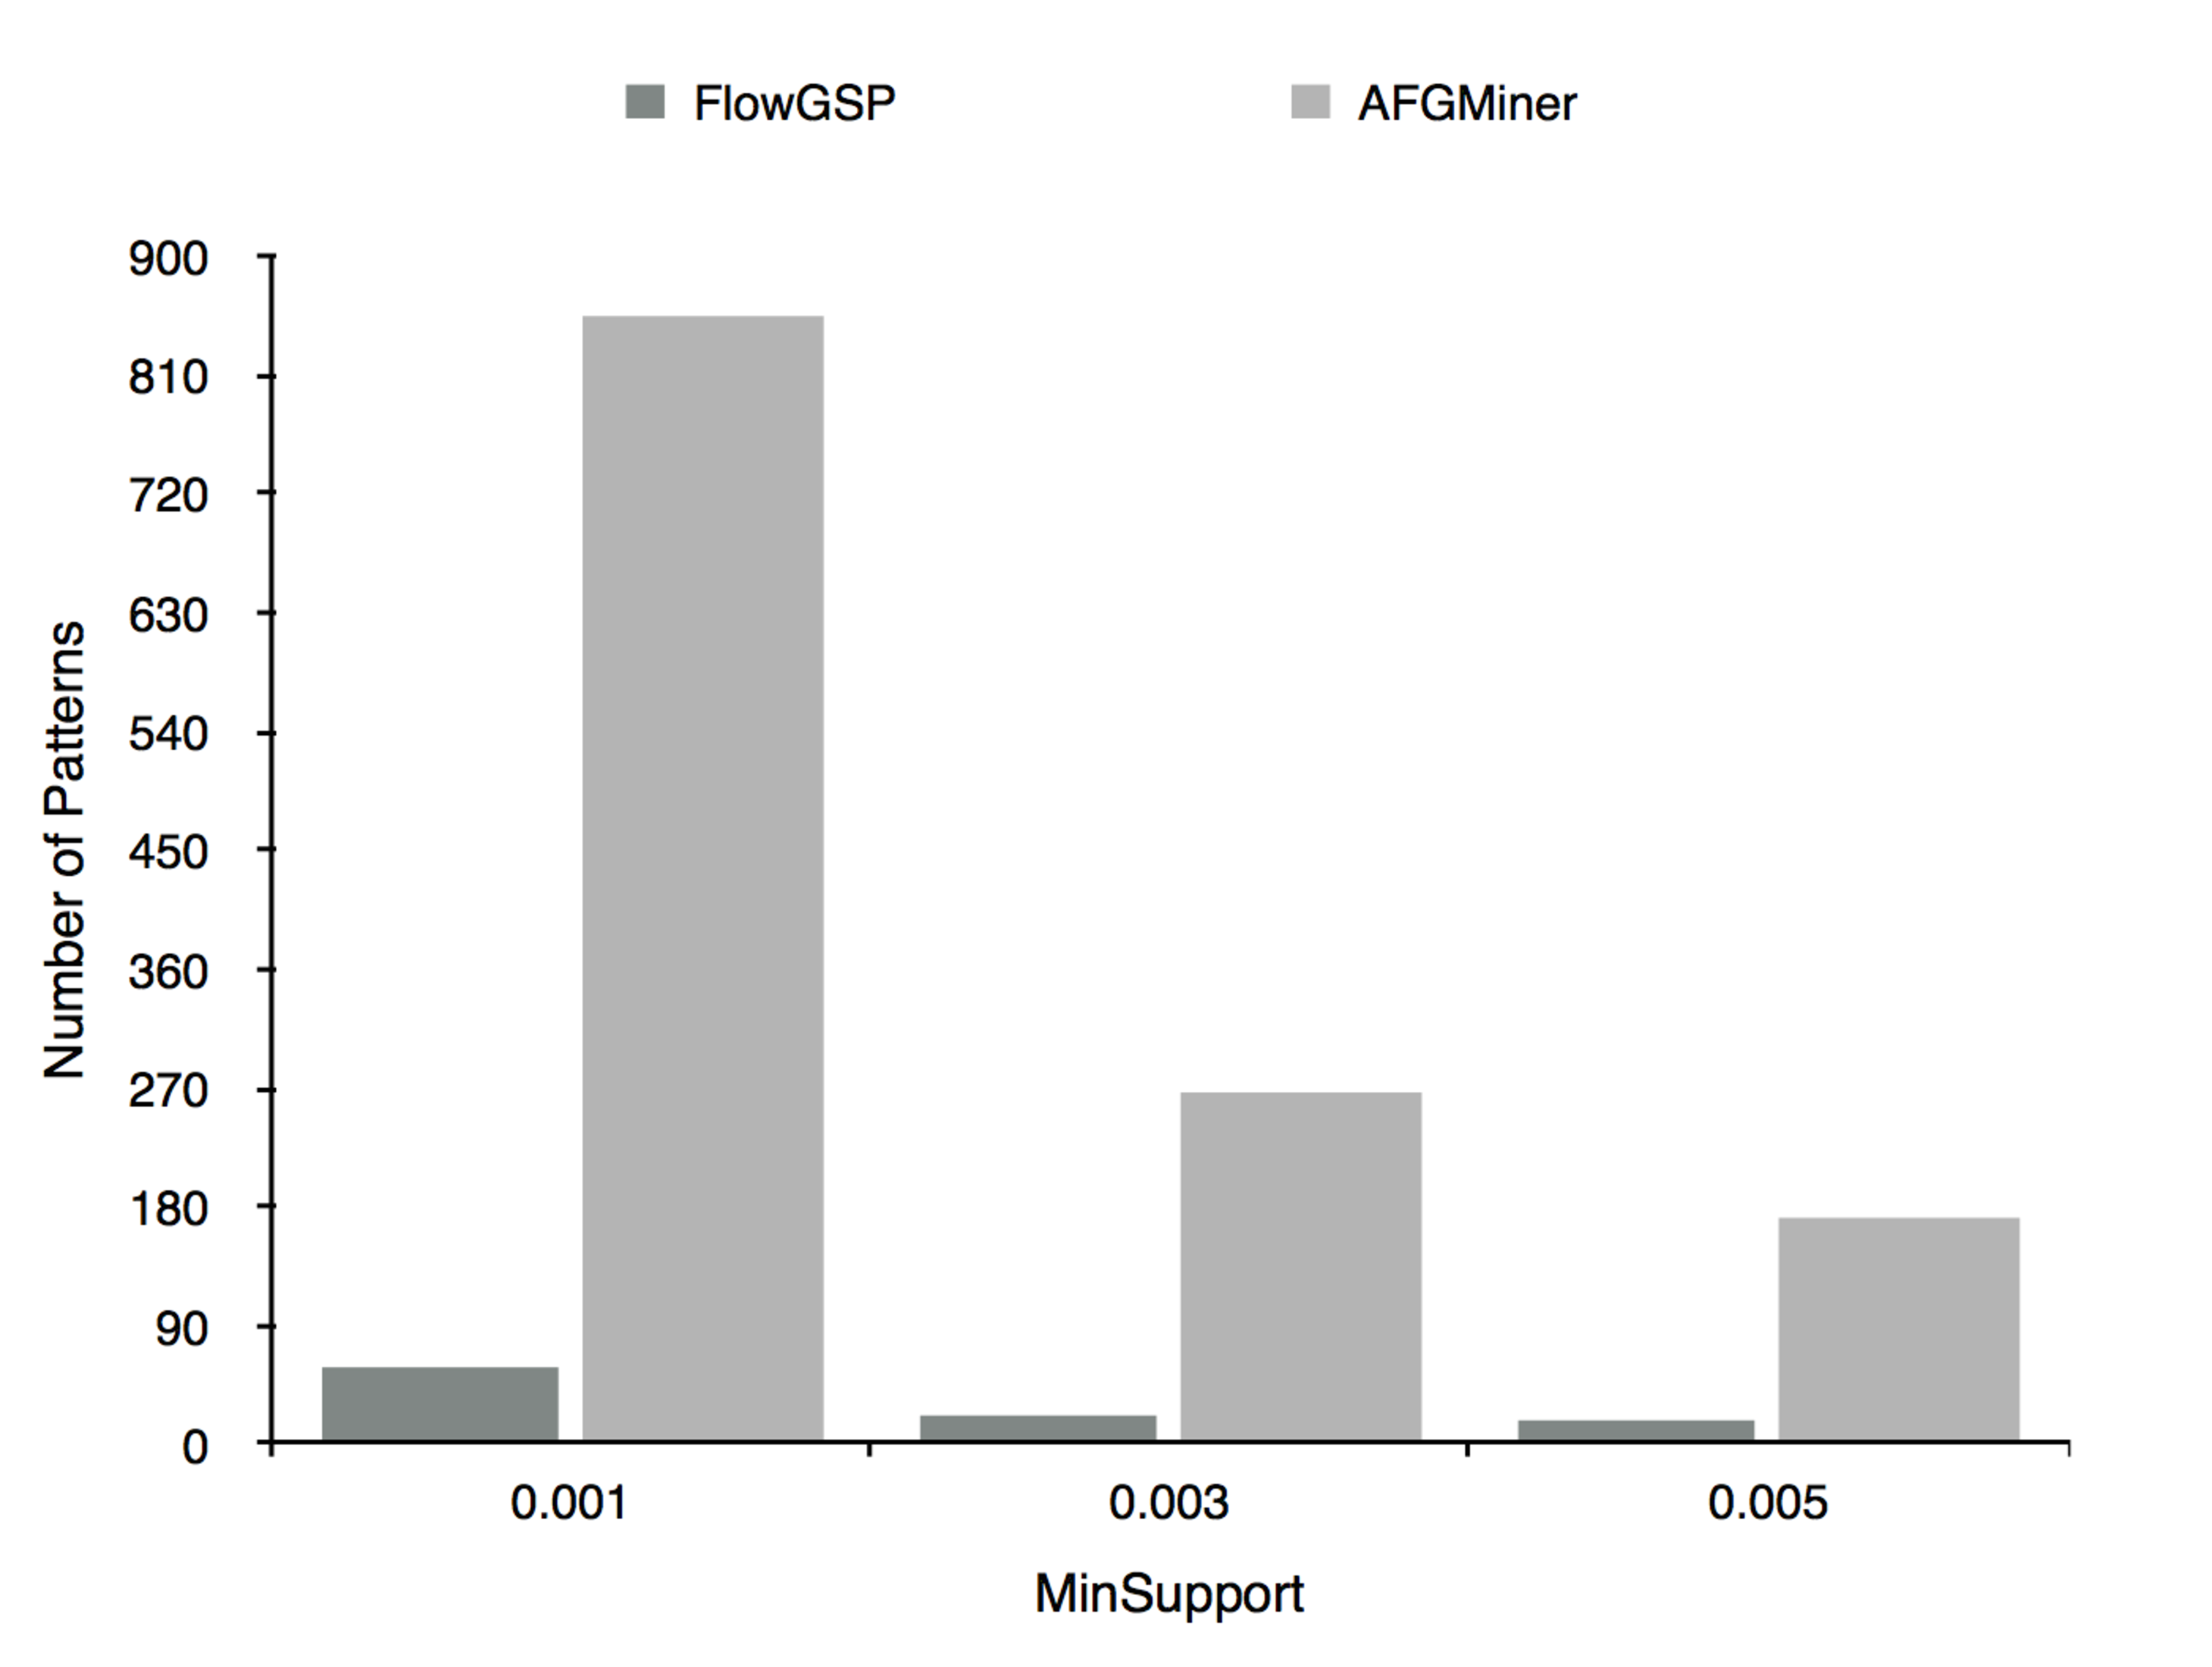
\includegraphics[scale=0.1]{figures/numPatternsComp.pdf}
    \caption{Patterns found by FlowGSP and AFGMiner}
    \label{fig:NumPatterns}
\end{figure}

Relevant observations from the experiments are:

\begin{enumerate}
\item The MaxAttrs value is not as relevant a factor in the run-time performance of AFGMiner as the number of EFG nodes visited during the mining process.
\item The run-time of AFGMiner increases moderately with the number of EFG nodes visited.
\item Although increasing the number of threads logically decreases run-time, there is a diminishing effect as MinSup/MMH increase, as time spent on data loading and temporary bookkeeping of patterns and pattern occurrences - both done serially by p-AFGMiner - start dominating the total run-time.
\end{enumerate}

\begin{figure}[h!]
\centering
    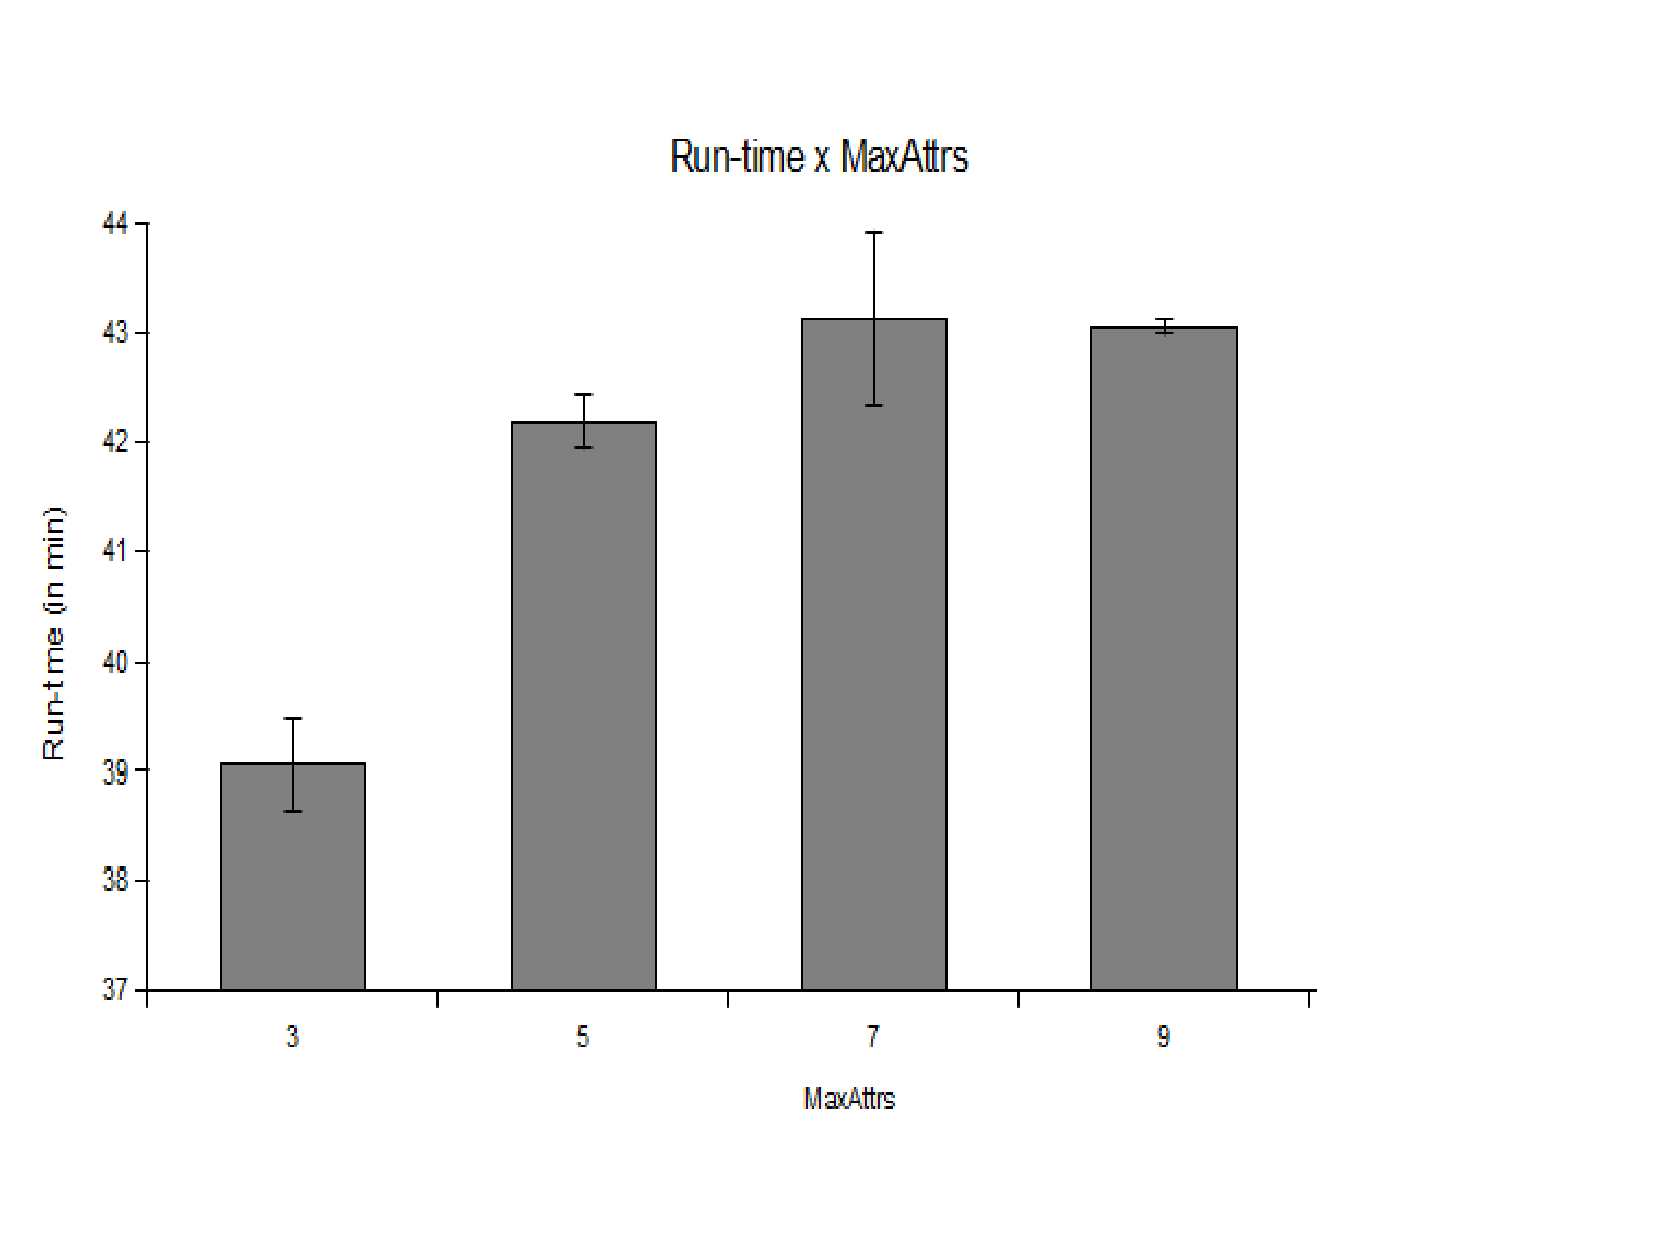
\includegraphics[scale=0.2]{figures/plot2.pdf}
    \caption{Experiment A.}
    \label{fig:Plot2}  
\end{figure}

\begin{figure}[h!]
\centering
    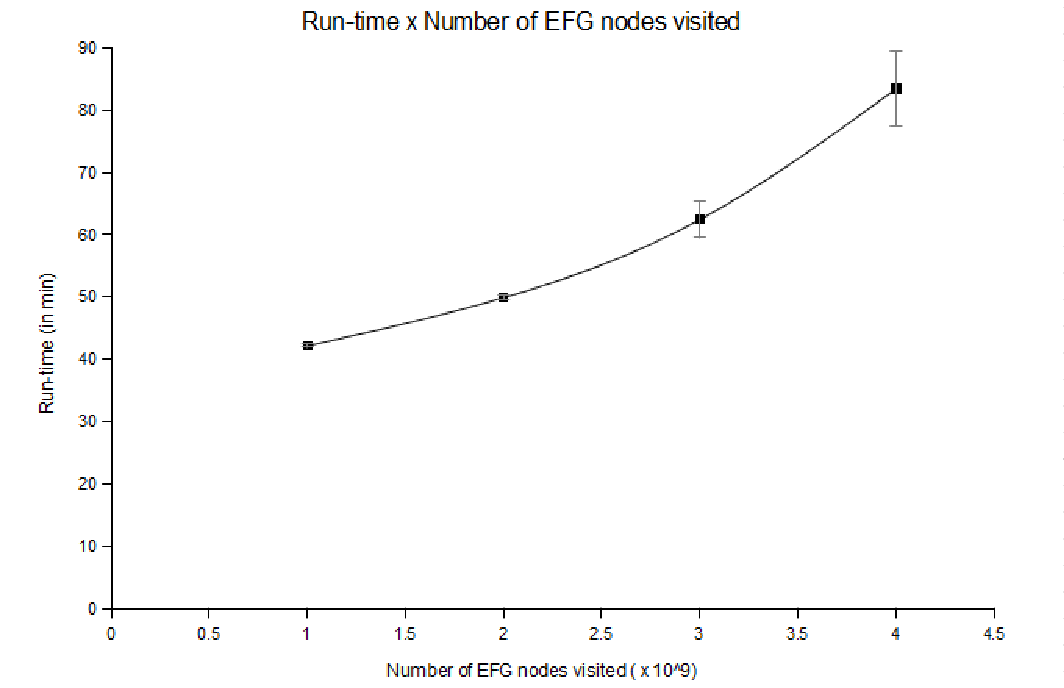
\includegraphics[scale=0.25]{figures/plot1.pdf}
    \caption{Experiment B.}
    \label{fig:Plot1}  
\end{figure}

\begin{figure}[h!]
\centering
    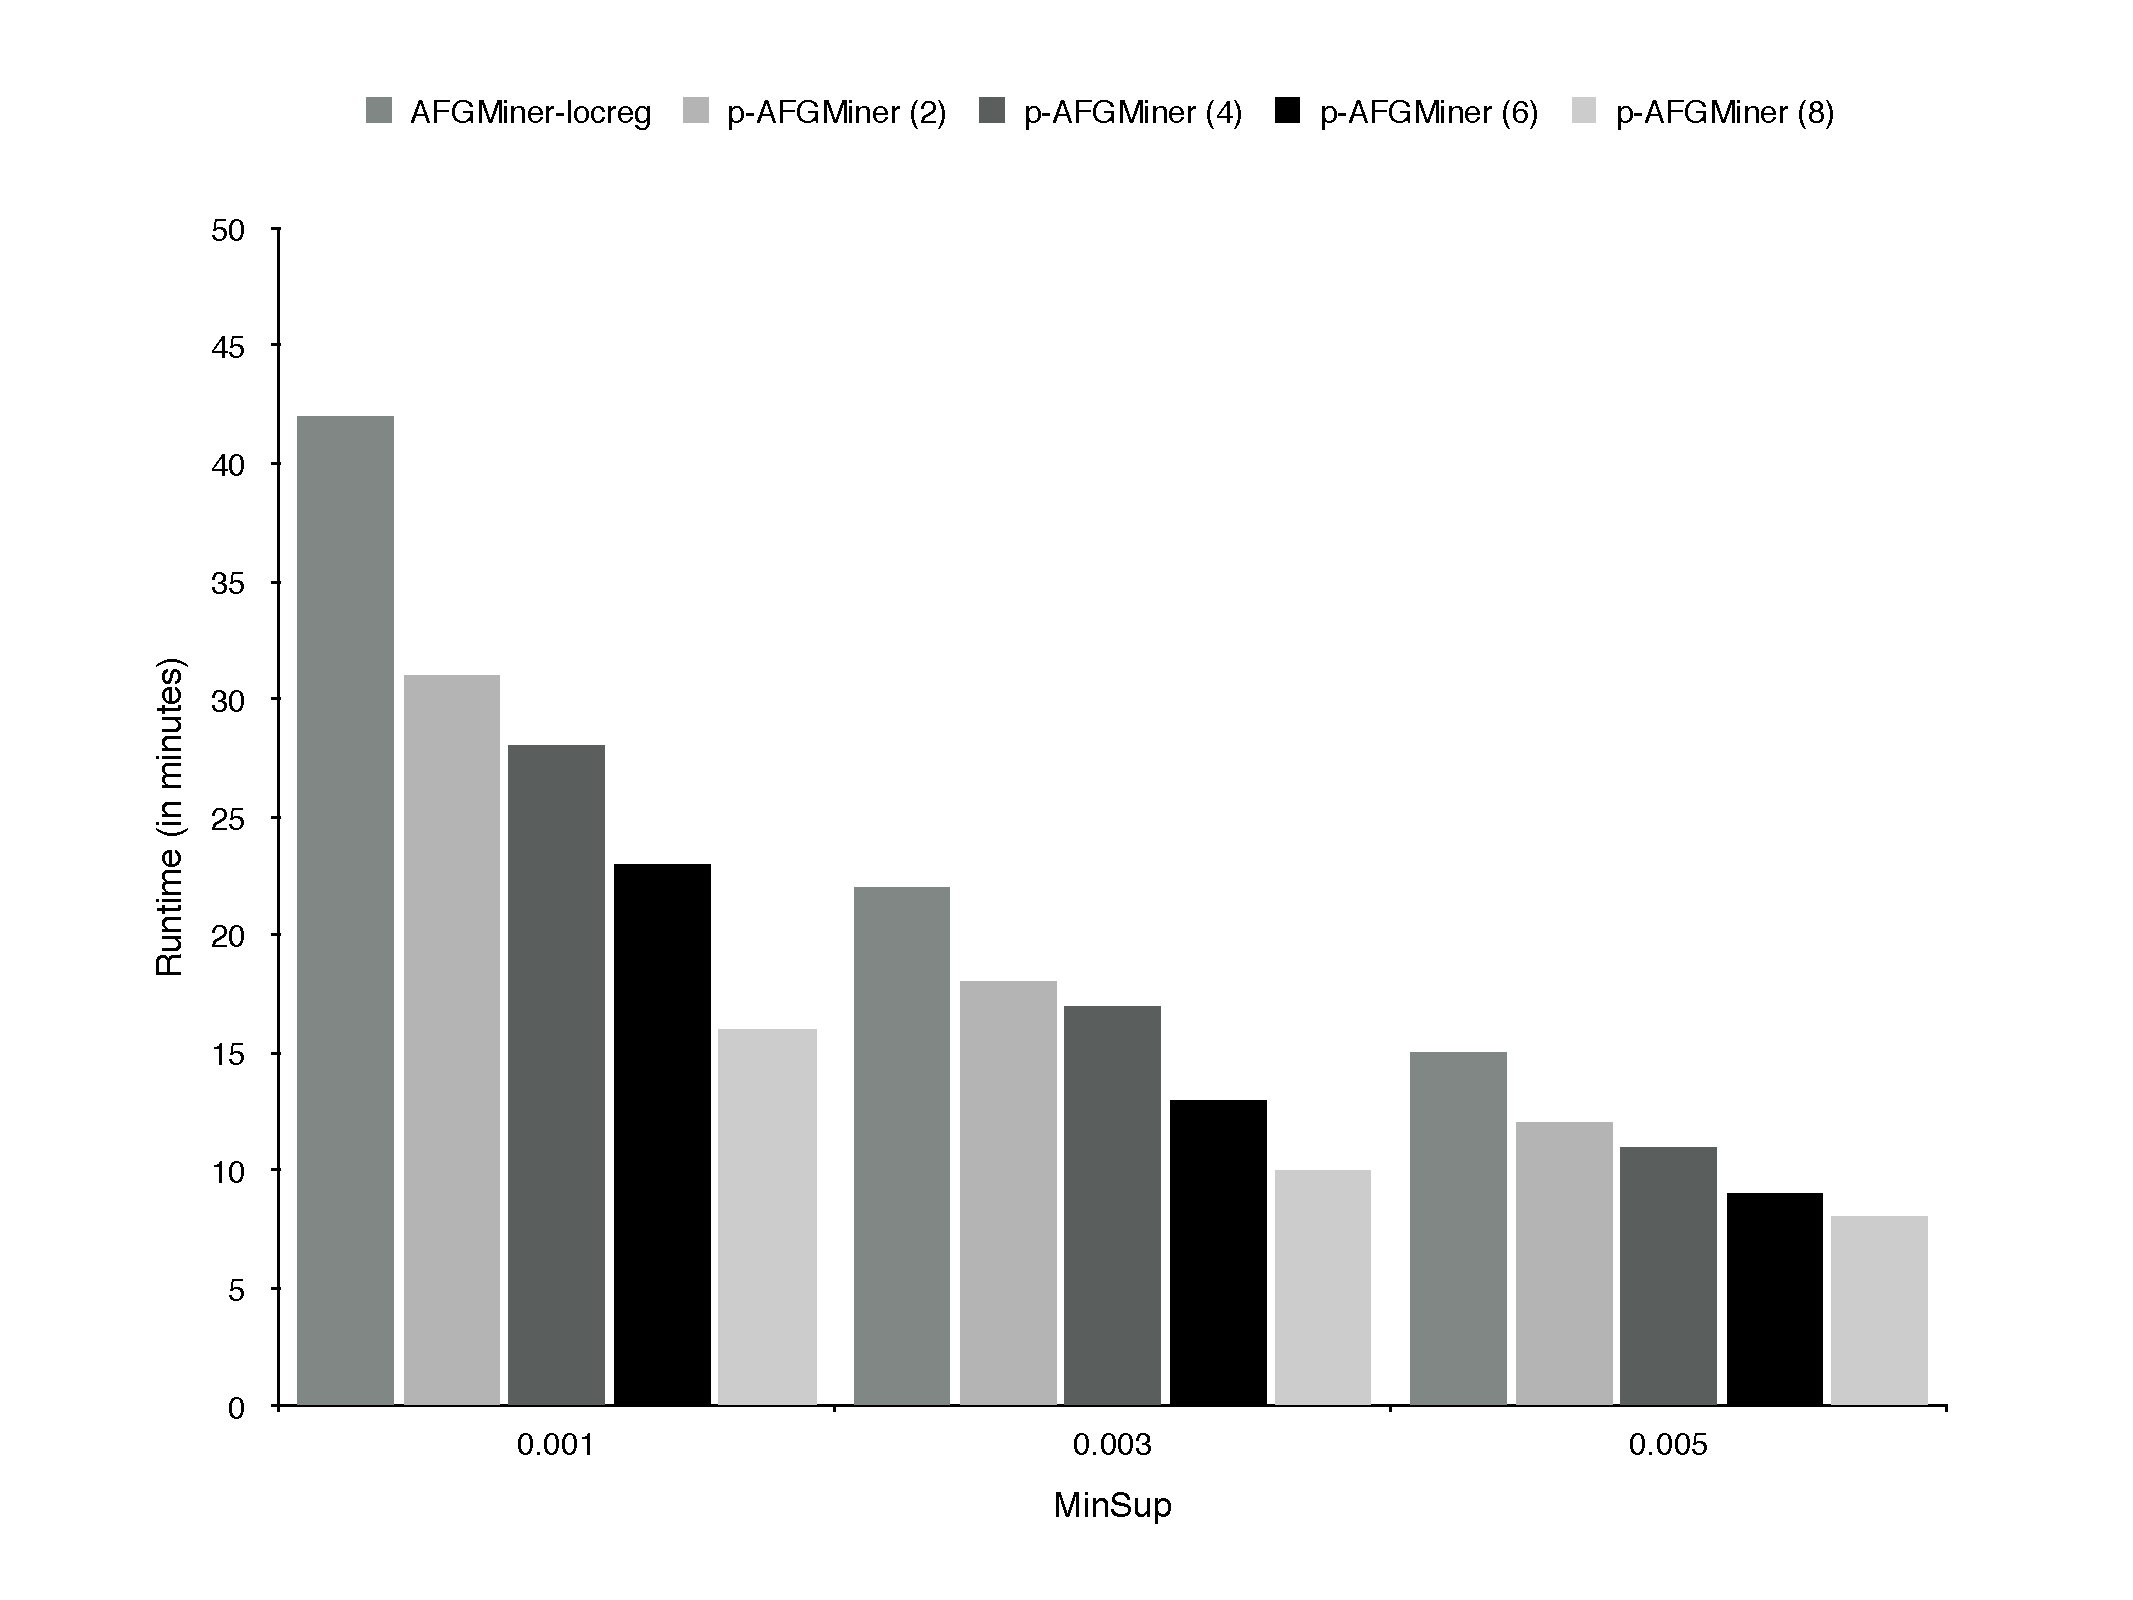
\includegraphics[scale=0.2]{figures/experimentC.pdf}
    \caption{Experiment C.}
    \label{fig:Plot3}  
\end{figure}

\begin{figure}[h!]
\centering
    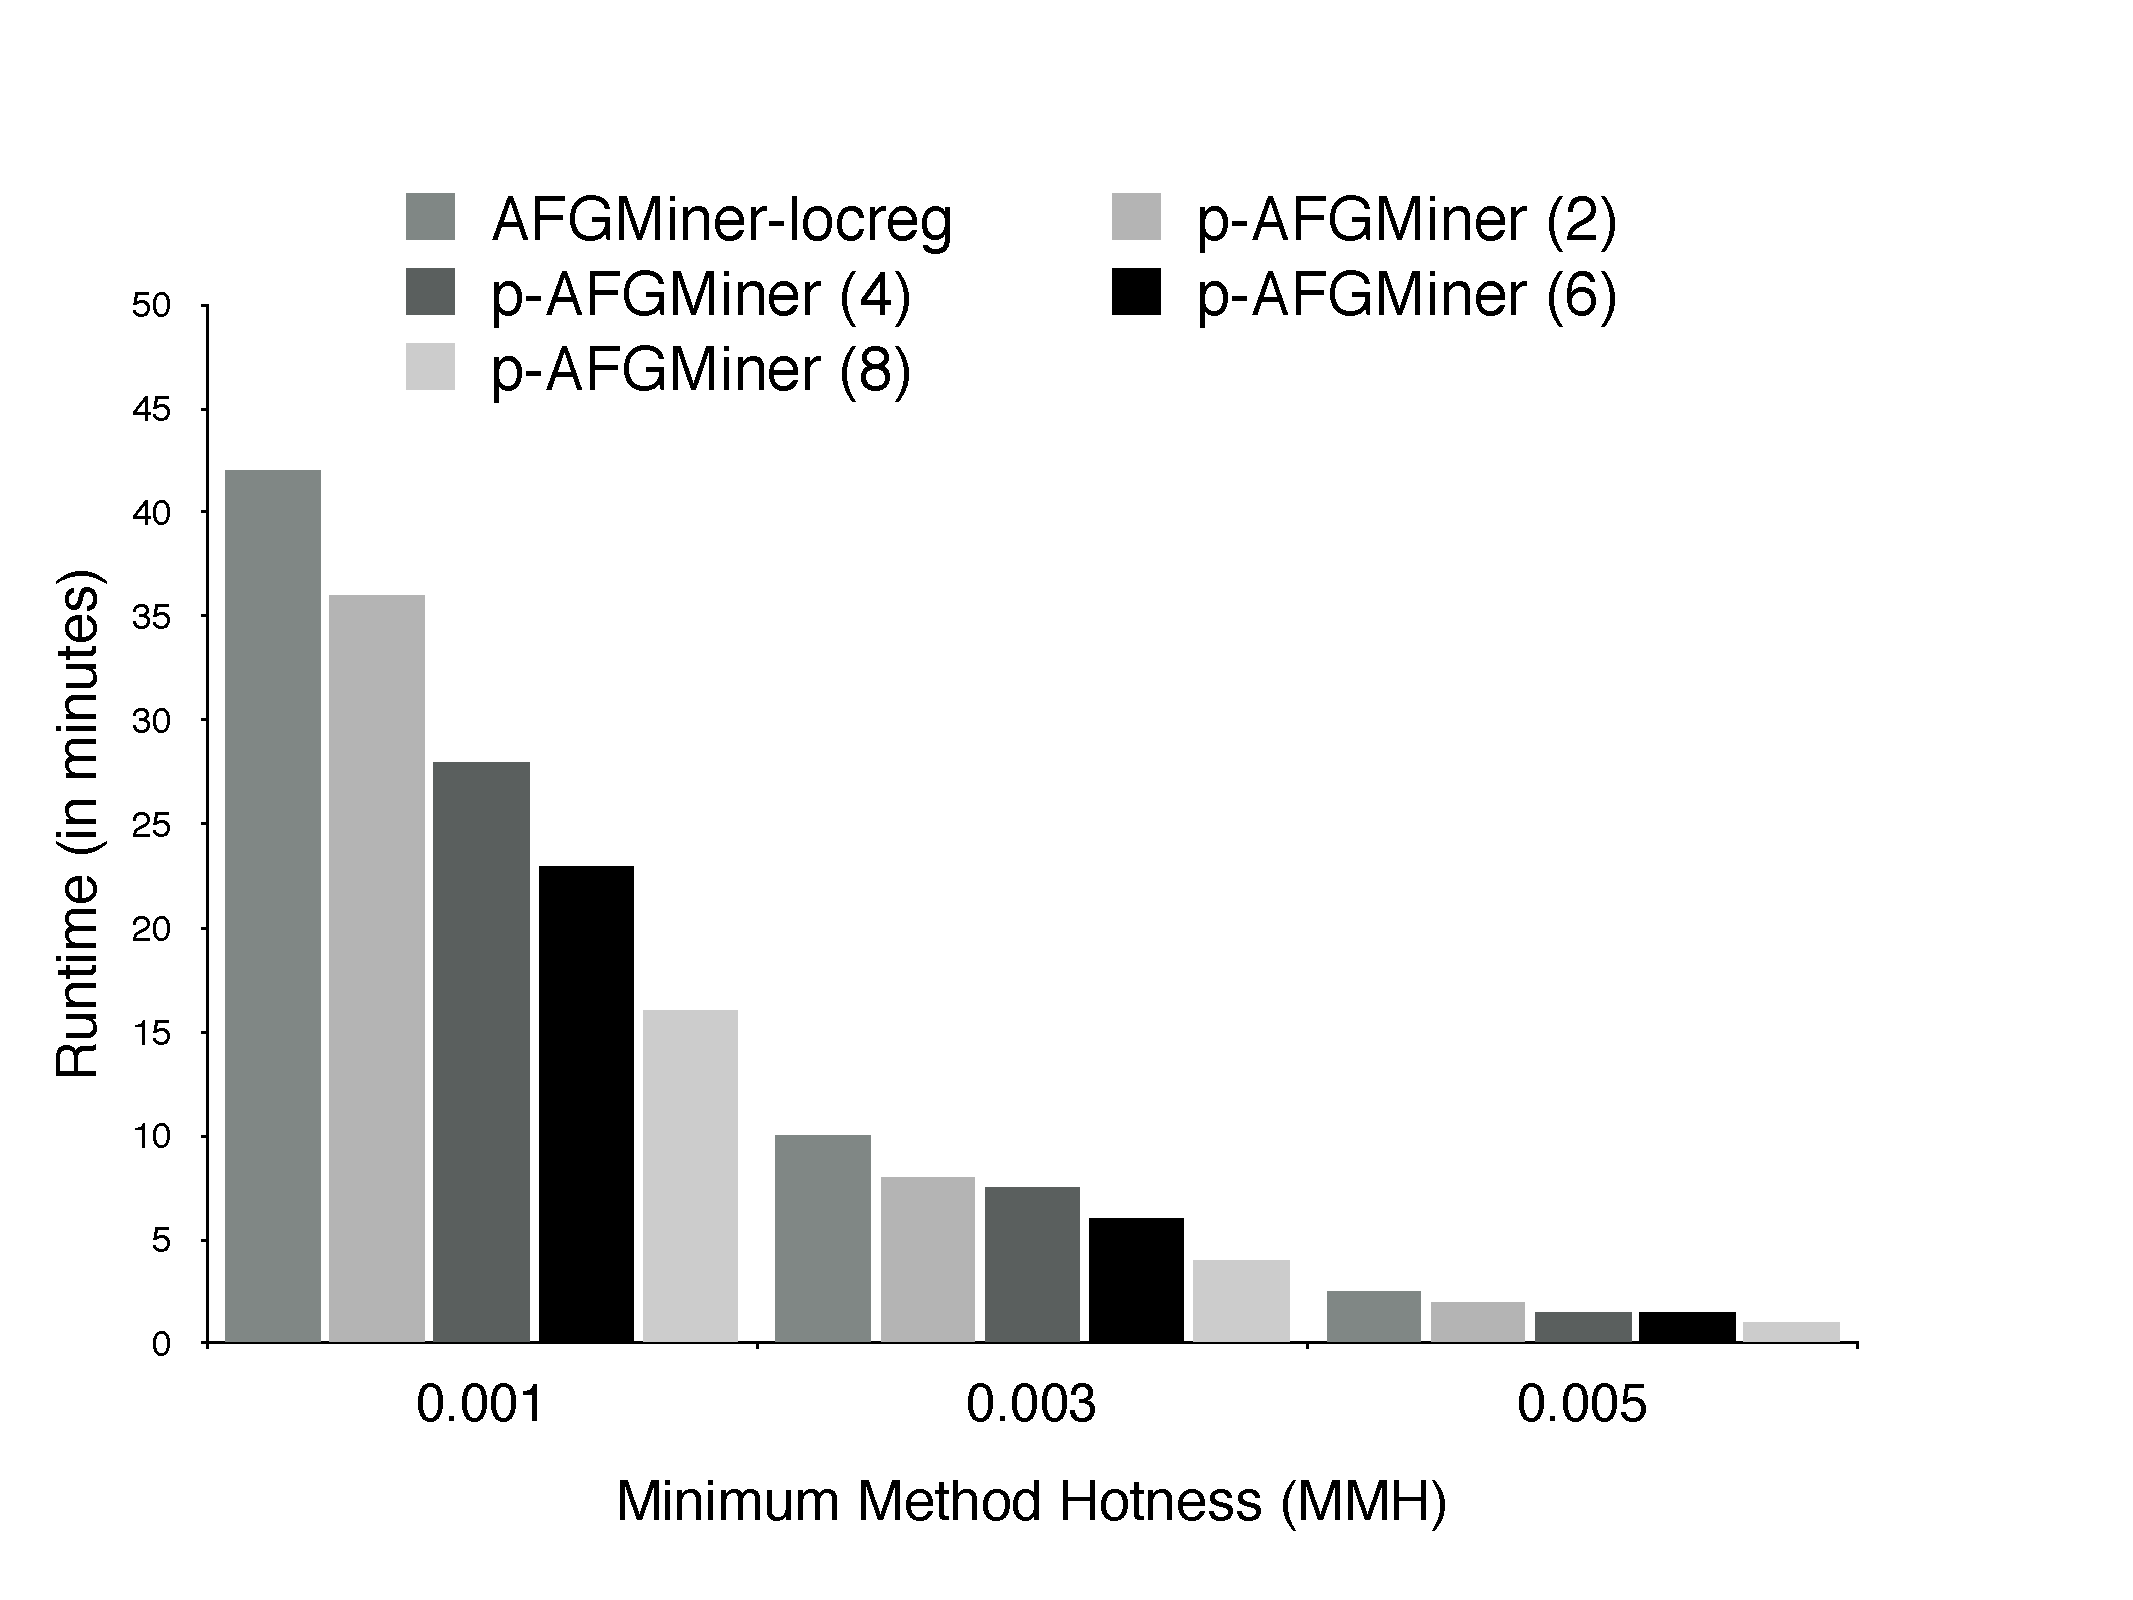
\includegraphics[scale=0.2]{figures/experimentD.pdf}
    \caption{Experiment D.}
    \label{fig:Plot4}  
\end{figure}
